\documentclass{beamer}

\usecolortheme[light]{solarized}

\beamertemplatenavigationsymbolsempty


\usepackage{booktabs}
\usepackage{graphicx}
\usepackage{hyperref}
\usepackage{minted}
\usepackage{moresize}
\usepackage{centernot}
\usepackage{standalone}
\usepackage{tcolorbox}
\usepackage{tikz}
\usepackage[normalem]{ulem}
\usepackage{xpatch}
\usepackage{fix-cm}

\xpatchcmd{\sout}
  {\bgroup}
    {\bgroup\def\ULthickness{2pt}}
      {}{}

\usetikzlibrary{calc, patterns}
\usetikzlibrary{arrows}
\usetikzlibrary{decorations.markings}
\usetikzlibrary{decorations.text}

\definecolor{twitter}{RGB}{64, 153, 255}
\definecolor{github}{RGB}{211, 211, 211}

\begin{document}

    \begin{frame}
        \begin{center}
            \Huge
                Will I have enough Mana?

               \vfill

            \Large
               Vince: \href{https://twitter.com/drvinceknight}{@drvinceknight}\\
        \end{center}

        % Hello, this will be a talk about a small python library called
        % "Ertai".
    \end{frame}

    \begin{frame}
               \begin{columns}
                   \begin{column}{.45\textwidth}
                       \begin{center}
                       
\includegraphics[height=3cm]{./img/CUident_CMYK/main.eps}
                       \end{center}

                       \begin{center}
                       
\includegraphics[height=3cm]{./img/axelrod_logo/main.png}
                       \end{center}
                   \end{column}
                   \begin{column}{.45\textwidth}
                       \begin{center}
                       
\includegraphics[height=3cm]{./img/ssi-logo/main.png}
                       \end{center}

                       \pause
                       \begin{center}
                       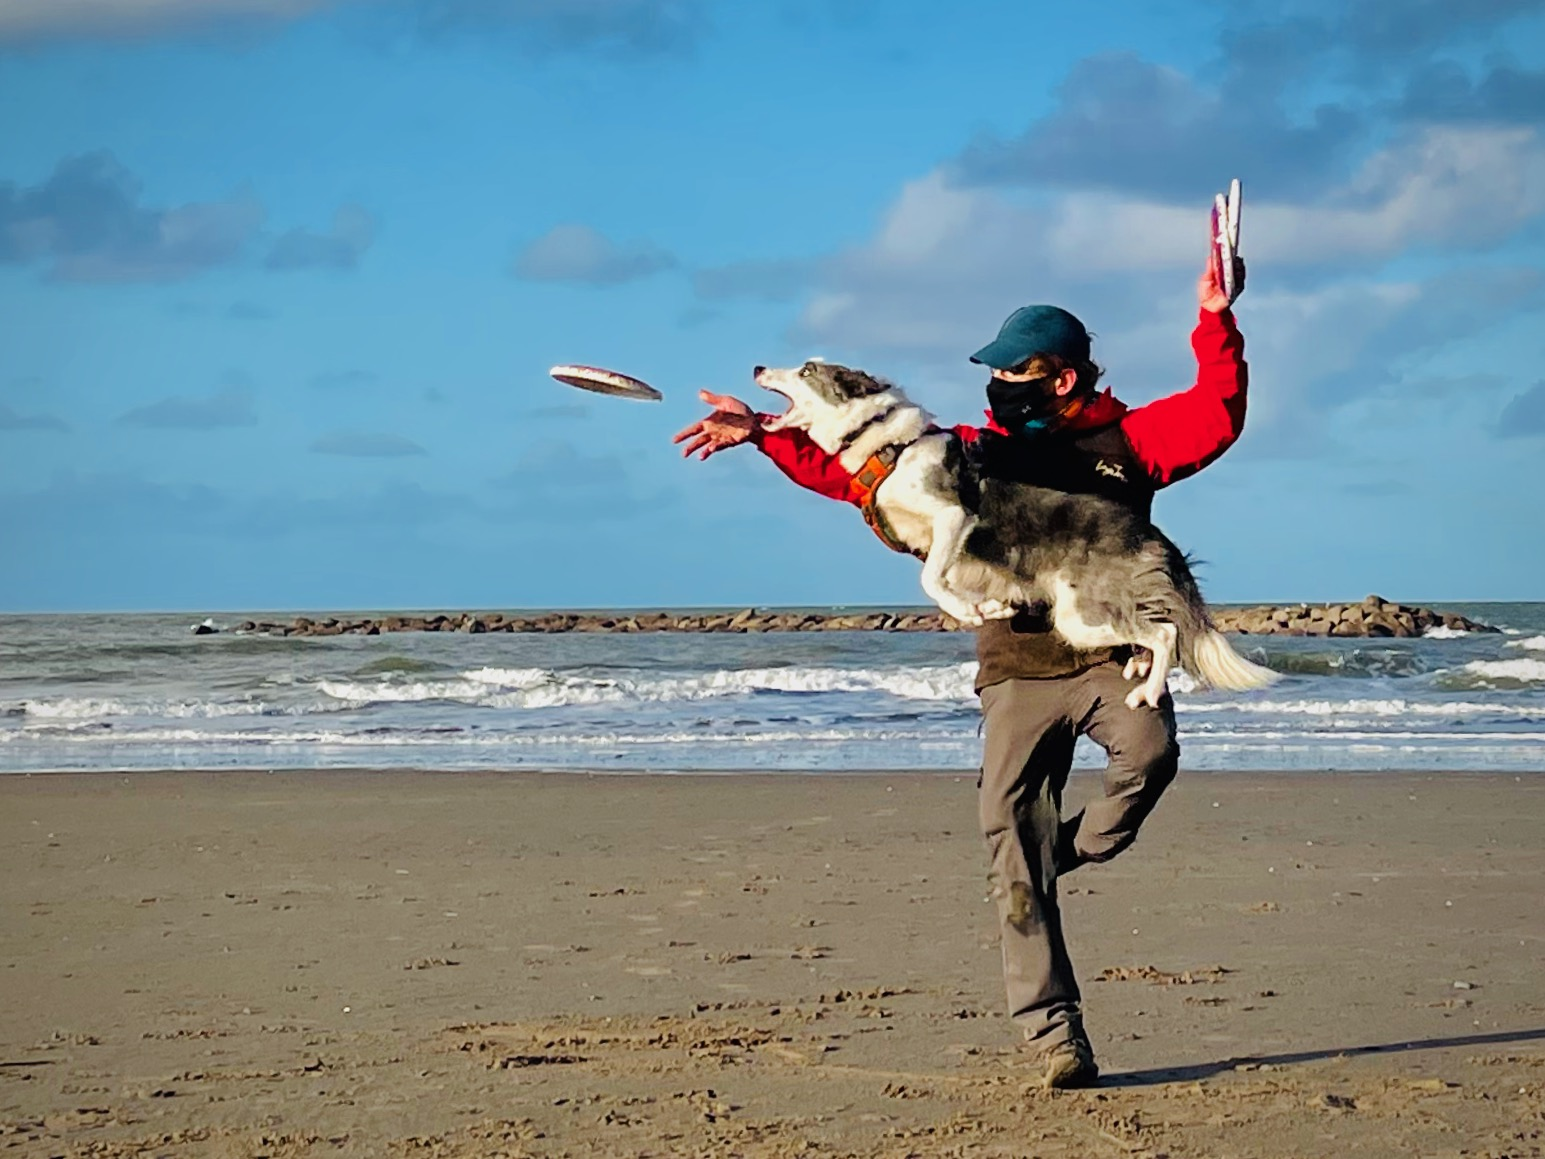
\includegraphics[trim={15cm 0 0 0}, clip, height=3cm]{./img/discdog/main.jpg}
                       \end{center}
                   \end{column}
               \end{columns}
    \end{frame}

    \begin{frame}
        \begin{center}
            
\includegraphics[width=.7\textwidth]{./img/nik_and_i/main.jpg}
        \end{center}
    \end{frame}

    \begin{frame}
        \begin{center}
            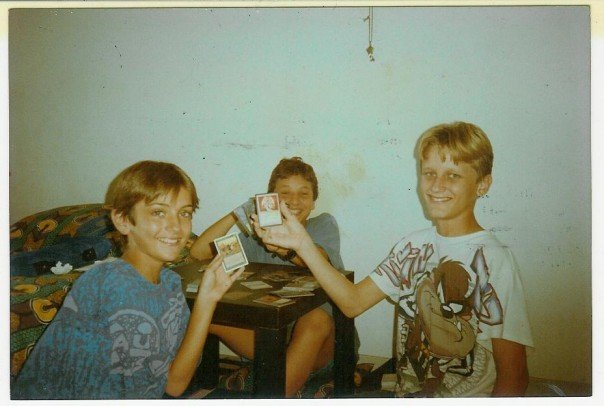
\includegraphics[width=.8\textwidth]{./img/young_me_playing_magic/main.jpg}
        \end{center}

        % My name is Vince, I'm the one on the right in the photo...
    \end{frame}

    \begin{frame}
        \begin{center}
            \Huge
            Magic The Gathering
        \end{center}
    \end{frame}

    \begin{frame}
        \begin{center}
            
\includegraphics[width=.8\textwidth]{./img/magic_battlefield/main.png}
        \end{center}
        \tiny{From: \url{https://magic.wizards.com/en/magic-gameplay}}
    \end{frame}

    \begin{frame}
        \begin{center}
            
\includegraphics[height=.7\textwidth]{./img/serra_angel/main.png}
        \end{center}
        \tiny{From: \url{https://magic.wizards.com/en/magic-gameplay}}
    \end{frame}

    \begin{frame}
        \begin{center}
            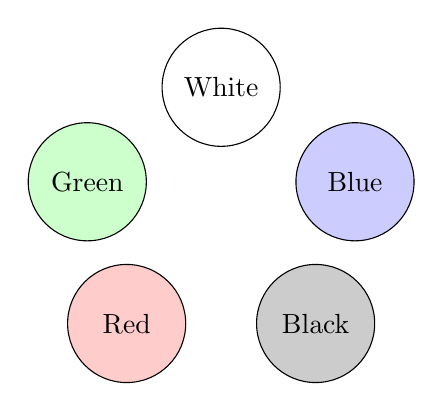
\begin{tikzpicture}
                \node [minimum size=1.5cm, circle, fill=white!20, draw] (We) at (0, 0) {White};
                \node [minimum size=1.5cm, circle, fill=blue!20, draw] (Be) at (1.7, -1.2) {Blue};
                \node [minimum size=1.5cm, circle, fill=black!20, draw] (Bk) at (1.2, -3) {Black};
                \node [minimum size=1.5cm, circle, fill=red!20, draw] (Rd) at (-1.2, -3) {Red};
                \node [minimum size=1.5cm, circle, fill=green!20, draw] (Gn) at (-1.7, -1.2) {Green};
            \end{tikzpicture}
        \end{center}
    \end{frame}


    \begin{frame}
        \begin{columns}
            \begin{column}{.5\textwidth}
                \begin{center}
                    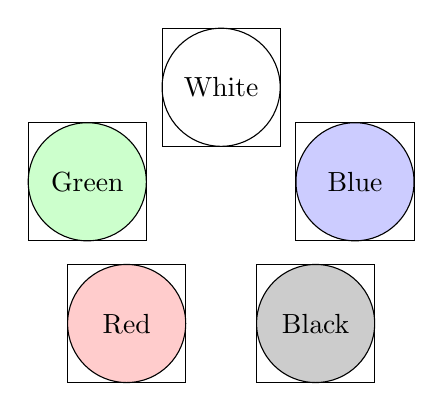
\begin{tikzpicture}
                        \node [minimum size=1.5cm, circle, fill=white!20, draw] (We) at (0, 0) {White};
                        \node [minimum size=1.5cm, circle, fill=blue!20, draw] (Be) at (1.7, -1.2) {Blue};
                        \node [minimum size=1.5cm, circle, fill=black!20, draw] (Bk) at (1.2, -3) {Black};
                        \node [minimum size=1.5cm, circle, fill=red!20, draw] (Rd) at (-1.2, -3) {Red};
                        \node [minimum size=1.5cm, circle, fill=green!20, draw] (Gn) at (-1.7, -1.2) {Green};

                        \onslide <1> {
                            \node [minimum size=1.5cm, draw] at (We) {};
                        }
                        \onslide <2> {
                            \node [minimum size=1.5cm, draw] at (Gn) {};
                        }
                        \onslide <3> {
                            \node [minimum size=1.5cm, draw] at (Rd) {};
                        }
                        \onslide <4> {
                            \node [minimum size=1.5cm, draw] at (Bk) {};
                        }
                        \onslide <5> {
                            \node [minimum size=1.5cm, draw] at (Be) {};
                        }
                    \end{tikzpicture}
                \end{center}
            \end{column}
            \begin{column}{.5\textwidth}
                \only <1> {
                    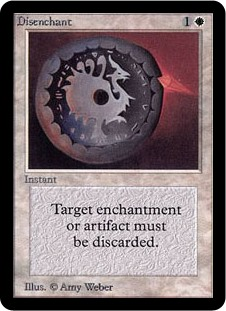
\includegraphics[width=\textwidth] {./img/disenchant/main.jpg}
                }
                \only <2> {
                    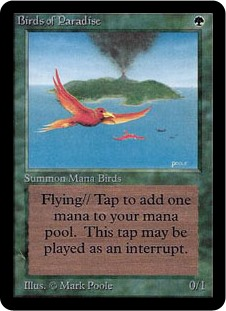
\includegraphics[width=\textwidth] {./img/bird_of_paradise/main.jpg}
                }
                \only <3> {
                    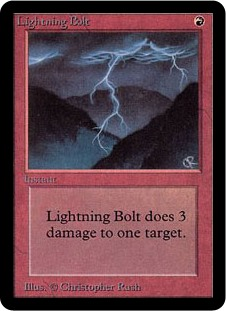
\includegraphics[width=\textwidth] {./img/lightning_bolt/main.jpg}
                }
                \only <4> {
                    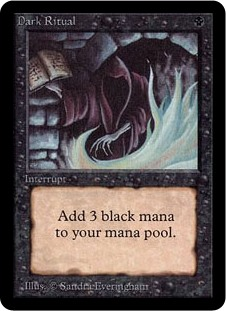
\includegraphics[width=\textwidth] {./img/dark_ritual/main.jpg}
                }
                \only <5> {
                    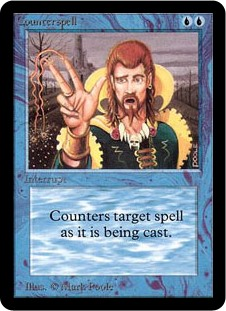
\includegraphics[width=\textwidth] {./img/counterspell/main.jpg}
                }
                \tiny{From: \url{https://gatherer.wizards.com}}
            \end{column}
        \end{columns}
    \end{frame}

    \begin{frame}
        \begin{center}
            \Huge
            Magic Demo
        \end{center}
    \end{frame}

    \begin{frame}
        \begin{center}
            \Huge
            Code Demo
        \end{center}
    \end{frame}

    \begin{frame}[fragile]
        \begin{columns}
            \begin{column}{.5\textwidth}
                \begin{center}
                    
\includegraphics[height=.8\textwidth]{./img/serra_angel/main.png}
                \end{center}
            \end{column}
            \tiny
            \begin{column}{.5\textwidth}
                \begin{minted}{python}
@dataclass
class Card:
    """A class for a base card."""

    title: Union[str, None] = None
    cost: Mana = Mana()
    tapped: bool = False

    def tap(self) -> None:
        """A method to tap a card"""
        self.tapped = True

    def untap(self) -> None:
        """A method to untap a card"""
        self.tapped = False

    def cast(self, pool: Mana) -> Mana:
        """
        A method to cast a card.
        Parameters:
            - pool: a mana pool
        It returns the pool after casting it.
        If there is insufficient mana in
        the pool the pool will be unmodified.
        """
        if self.cost <= pool:
            pool -= self.cost
        return pool
                \end{minted}
            \end{column}
        \end{columns}
    \end{frame}

    \begin{frame}
        \begin{center}
            \scalebox{.7}{\documentclass{beamer}

\usecolortheme[light]{solarized}

\beamertemplatenavigationsymbolsempty

\usepackage{hyperref}

\usepackage{tikz}
\usetikzlibrary{calc}

\begin{document}

\begin{center}


    \begin{tikzpicture}
        \draw [thick] (0,-4) -- (0, 4);
        \draw [thick] (-5,0) -- (5, 0);

        \node at (-2, 2) {Tutorials};
        \node at (2, 2) {How To's};
        \node at (-2, -2) {Discussions};
        \node at (2, -2) {Reference};
    \end{tikzpicture}

\href{"https://twitter.com/evildmp"}{@EVILDMP}

\end{center}



\end{document}
}
        \end{center}
        \tiny{With: \texttt{@GeraintPalmer} and \texttt{@NikoletaGlyn}}
    \end{frame}

    \begin{frame}
        \Huge
        \begin{center}
            \texttt{src/}
        \end{center}
    \end{frame}

    \begin{frame}
        \Huge
        \begin{center}
            \texttt{tests/}
        \end{center}
    \end{frame}

    \begin{frame}
        \Huge
        \begin{center}
            \texttt{README.md}
        \end{center}
    \end{frame}

    \begin{frame}
        \large
        Anton Zhiyanov:
        \begin{center}
            \textbf{How to make an awesome Python package in 2021}
        \end{center}
        \tiny
        \hfill
        \url{https://antonz.org/python-packaging/}
    \end{frame}

    \begin{frame}
        \large
        Daniele Procida
        \begin{center}
            \textbf{Diátaxis Framework - A Systematic Framework For Technical Documentation Authoring.}
        \end{center}
        \tiny
        \hfill
        \url{https://diataxis.fr}
    \end{frame}

    \begin{frame}
        \begin{center}
            \Huge
            Will I have enough mana?
        \end{center}
    \end{frame}

    \begin{frame}
        \Large
        \begin{center}
            \texttt{python -m pip install ertai}
        \end{center}

        \begin{center}
            \url{https://github.com/drvinceknight/ertai/} (PRs welcome)
        \end{center}

        \begin{center}
            \url{https://antonz.org/python-packaging/}
        \end{center}

        \begin{center}
            \url{https://diataxis.fr}
        \end{center}

        \begin{center}
            \url{https://magic.wizards.com/}
        \end{center}


        \begin{center}
            \texttt{@drvinceknight}
        \end{center}
    \end{frame}

\end{document}
